Dựa trên những ý tưởng từ trước đến nay, nhiệm vụ của nhóm tác giả thực hiện học tăng cường để giải quyết bài toán tìm đường đi ngắn nhất cho môi trường môi trường nhất định. Mặc dù có rất nhiều cách tiếp cận, đặc biệt khi sự ra đời của nhiều thuật toán trong lĩnh vực AI, khóa luận thu hẹp lại khi giải quyết bài toán với \word{Q-learning Cơ bản}{Vanilla Q-learning}, có thể tiền đề cho các nghiên cứu trong tương lai.\\
\\
Một vài thử nghiệm được thực hiện bởi \cite{WHG_yasyf}  được nhóm lấy cảm hứng và thực hiện lại. Khi \citeauthor{WHG_yasyf} thử hiện trên môi trường flash rất khó khăn khi tốn nhiều thời gian tùy chỉnh môi trường trên trình duyệt. Nhóm tác giả đã tìm phương án thay thế tốt hơn để thực nghiệm.\\
\\
Một số các vấn đề liên quan bao gồm thực hiện  Q-learning từ các tương tác với môi trường. Các tùy chỉnh trên các mô hình giống nhau để đạt được sự hiểu biết "được gì và tại sao" là những kinh nghiệm tốt cho các nghiên cứu sau này.\\
\\
Để đạt được những điều trên, các tùy chỉnh về trạng thái, phần thưởng và một số tham số liên quan đến quá trình huấn luyện Q-learning được đề ra và thực hiện trên nhiều giả thuyết được đặt ra sau mỗi lần tùy chỉnh.
\section{Chuẩn bị môi trường}
\label{env_repair}
%need to continue
\subsection{Môi trường Java}
Mã nguồn của WHG được hoàn thiện rất tốt nên việc bỏ đi những phần dư thừa (âm thanh, phần mở đầu hay hướng dẫn và thread khiến cho trò chơi chậm lại) là cần thiết để giảm thiểu thời gian chạy của chương trình.\\
Nhóm tác giả sử dụng Python là "bộ não" của robot và Java để tạo môi trường cung cấp trạng thái để huấn luyện thì để trao đổi thông tin giữa ngôn ngữ Java và Python đơn giản nhất là ghi đè lên ổ đĩa, như hình \ref{fig:transfer_java_env}\\
\begin{figure}[h]
    \centering
    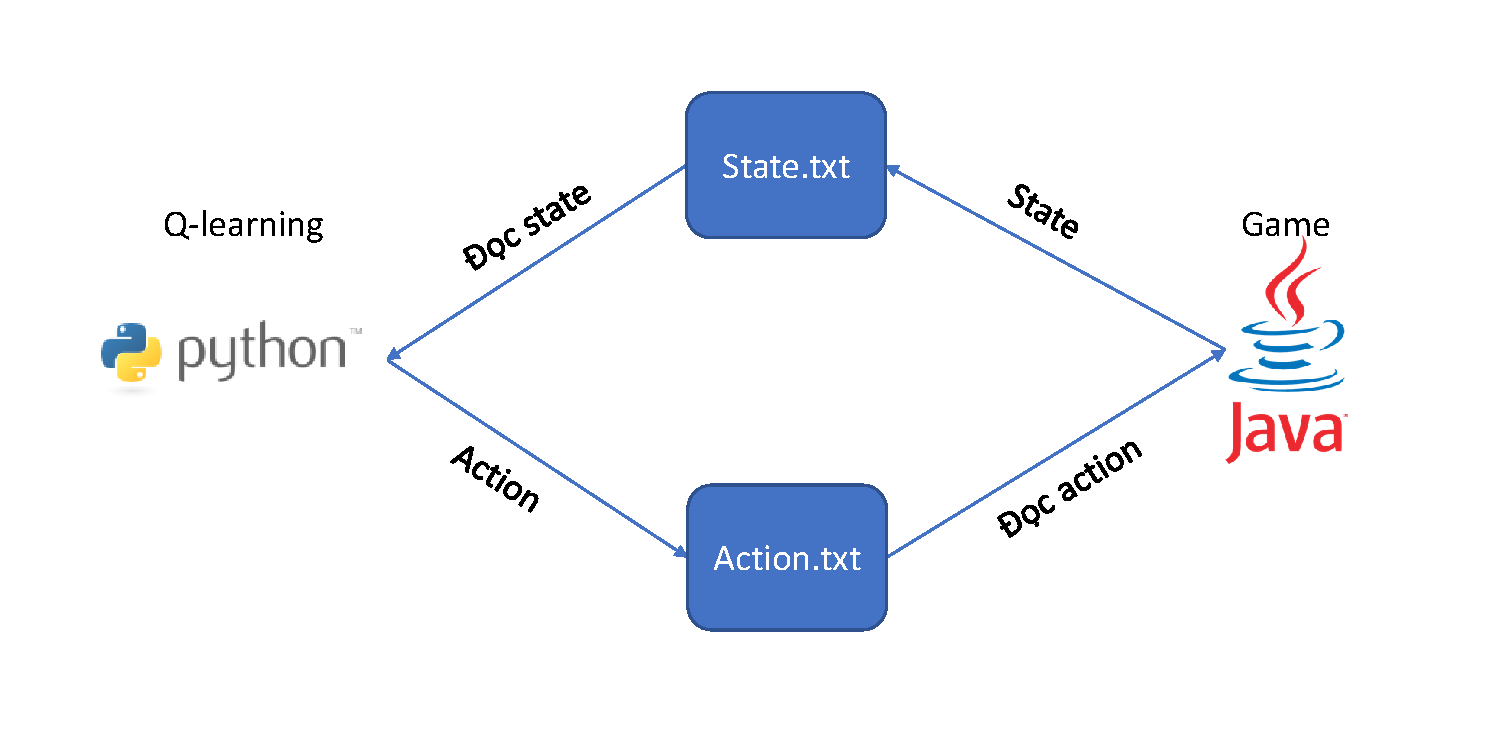
\includegraphics[width=130mm,scale=0.3]{Pic/transfer_java_env.pdf}
    \caption[Chuyển dữ liệu giữa Python và Java]{\textit{Chuyển dữ liệu giữa Python và Java}, mỗi bước thực hiện của robot được thực hiện theo thứ tự Python sẽ đọc trạng thái từ tập tin State.txt do Java cung cấp, sau đó trả về hành động được ghi vào tập tin Action.txt được Java đọc và tạo trạng thái tiếp theo.}
    \label{fig:transfer_java_env}
\end{figure}
Mô tả môi trường của World's Hardest Game (WHG) như sau:\label{begin_setting}
\begin{itemize}
    \item \textbf{Một tập trạng thái hữu hạn S}, mỗi trạng thái bao gồm vị trí của robot, vị trí của vật cản. Các vị trí này có nằm trên bản đồ kích thước 40x40.
    \item \textbf{Một tập hành động hữu hạn A},  có 5 hành động,  ($a_t=0$ : trái),  ($a_t=1$ : phải), ($a_t=2$ : lên), ($a_t=3$ : xuống), ($a_t=4$ : đứng yên).
    \item \textbf{Một hàm phần thưởng} $r = R(s_t, a_t, s_{t+1}$, đây là phần thưởng tức thời khi thực hiện hành động $a_t$: $r =1$ khi robot tới được đích, $r=-1$ khi robot đụng phải vật cản
\end{itemize}
Kiến trúc của mô hình khi chạy trên môi trường này giống giống như \cite{DBLP:journals/corr/MnihKSGAWR13} nhưng không dùng \word{Mạng nơ-ron tích chập}{Convolutional Neural Networks}.
\subsection{Môi trường Socket}
Sử dụng socket\cite{5232440} để trao đổi thông tin giữa ngôn ngữ Java và Python, với máy chủ sẽ là thuật toán Q-learning còn máy thành phần sẽ thực hiện chạy môi trường trò chơi trên Java. \\
\\
Đồng thời, nhóm tác giả đưa ra một bản đồ mới cho trò chơi, với các cài đặt đơn giản hơn, bé hơn, ít phức tạp hơn so với bản đồ gốc khi rút kinh nghiệm từ việc huấn luyện trên môi trường Java. Môi trường thay vì các bước đi của robot thay đổi theo từng pixel, chúng tôi đơn giản hóa bằng cách thay đổi mỗi bước đi sẽ theo từng ô, điều này được áp dụng cho cả vật cản. Việc cắt bớt phần vùng an toàn và vùng chiến thắng với mục đích robot sẽ "tình cờ" thắng nhiều hơn trong hình \ref{fig:1_step_new_env}
Tiến hành huấn luyện trên cả 2 môi trường trên và sử dụng kiến trúc ở môi trường Java
\begin{figure}[h]
    \centering
    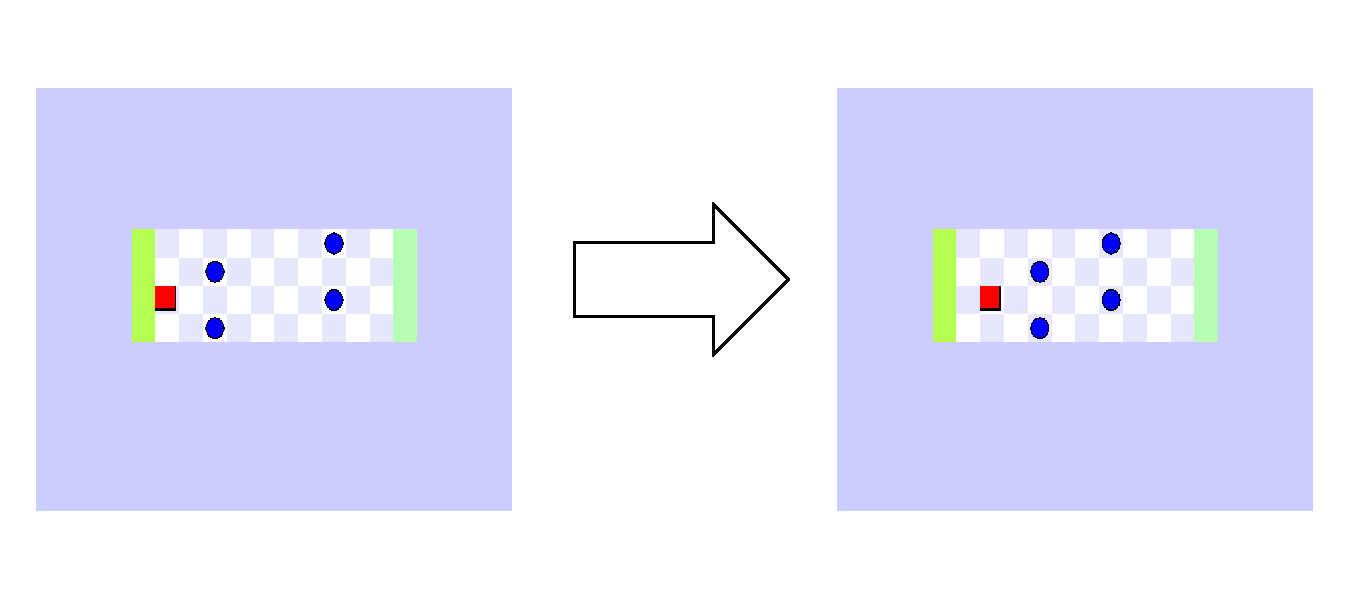
\includegraphics[width=150mm,scale=0.5]{Pic/1_step_new_env.pdf}
    \caption[Môi trường mới]{\textit{Môi trường mới}, robot thực hiện một bước (qua phải) trong môi trường mới theo từng ô thay vì từng pixel.}
    \label{fig:1_step_new_env}
\end{figure}
\subsection{Môi trường Python}
Khi môi trường lúc này của khóa luận lúc này trở nên đơn giản hơn so với môi trường gốc của WHG nên việc thực hiện lại  trò chơi trên ngôn ngữ Python không tốn nhiều thời gian. Với mục đích loại bỏ thời gian tạo hình ảnh và môi trường dễ tùy biến cho tính chất của khóa luận là điều cần thiết.\\
\section{Mô hình cơ sở}\label{baseline_model}
\subsection{Điều chỉnh trạng thái}
Khi thực hiện lại trên môi trường mới với các cài đặt như \ref{begin_setting}, nhóm tác giả thu được kết quả tệ do đó việc tìm hiểu môi trường là cần thiết. Khi xét đến vị trí hoạt động của vật cản, chúng tôi đặt ra giả thiết khi robot gặp phải trạng thái giống nhau nhưng hướng đi của các vật cản là khác nhau, sẽ khiến robot "bối rối"  được biểu thị như hình \ref{fig:conflict_enemy_position} . Do đó khi ra quyết định trên dữ kiện hiện thời sẽ phải xác định hướng đi của các vật cản mà do tính chất "không nhớ" được đề cập trong \ref{MDP} thì robot phải "đoán" khi thực hiện việc học. Để khắc phục, nhóm tác giả bổ sung hướng đi của vật cản vào các trạng thái, sẽ được mô tả cụ thể trong phần \ref{change_state}.\\
\begin{figure}[h]
    \centering
    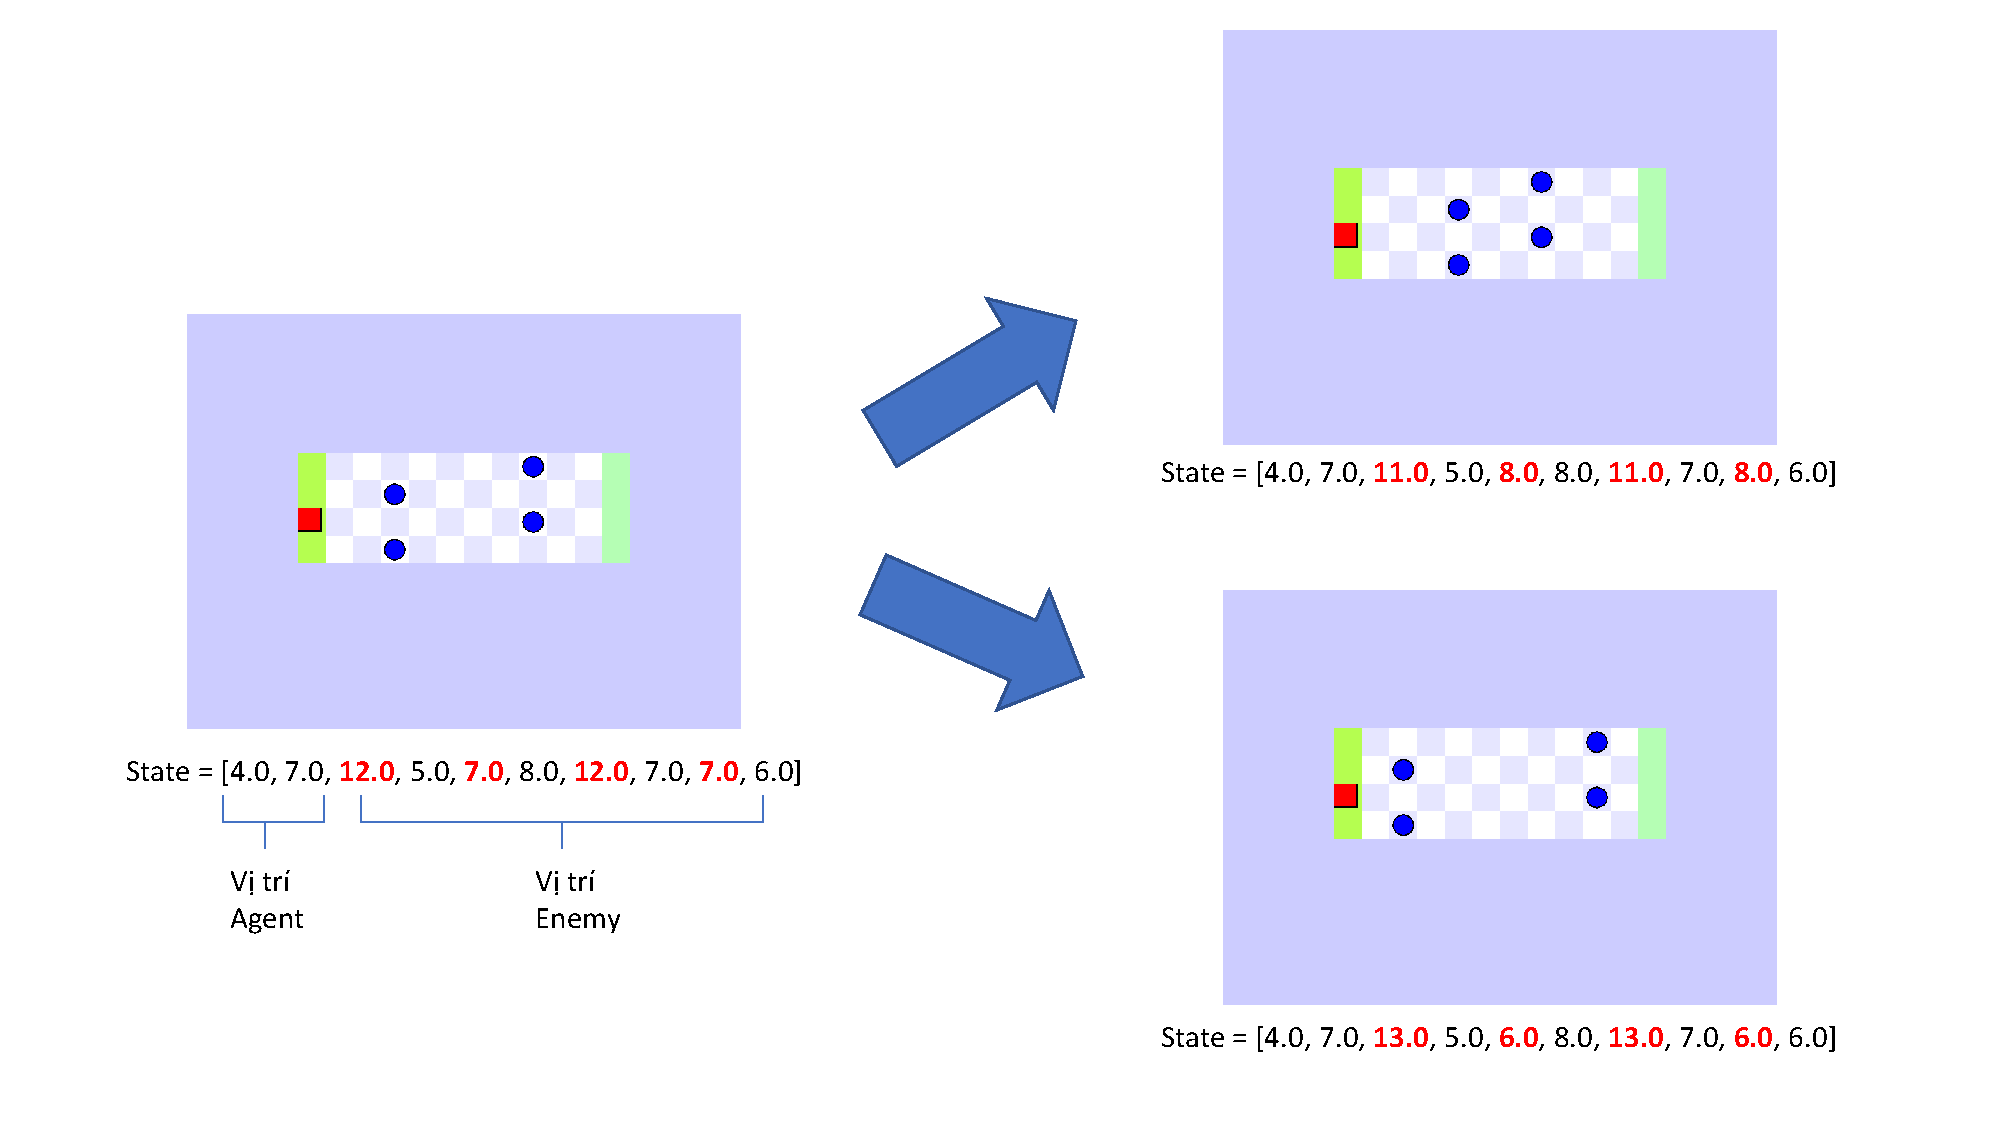
\includegraphics[width=150mm,scale=0.5]{./Pic/conflict_enemy_position.pdf}
    \caption[Đoán các trạng thái]{\textit{Đoán các trạng thái}, ví dụ của sự "rối bời" của robot khi chọn hành động giữa các sự biến đổi trạng thái. Khi gặp một trạng thái robot phải đoán bước tiếp theo của các vật cản, hình ở trên thể hiện vật cản ở vị trí hiện tại sang trái và ngược lại.}
    \label{fig:conflict_enemy_position}
\end{figure}
\subsection{Một số tùy biến tham khảo}\label{ref_app}
Sự thành công của \cite{DBLP:journals/corr/MnihKSGAWR13} là bước ngoặt trong lĩnh vực học tăng cường khi thực hiện thành công hai ý tưởng mà sau này được nghiên cứu và phát triển rất nhiều, đó là \word{Lịch sử kinh nghiệm}{Experience Replay}và \word{Mạng mục tiêu}{Target Network}.
\begin{itemize}
    \item \textbf{Lịch sử kinh nghiệm}, chứa kinh nghiệm của robot theo bộ $(s_t, a_t, s_{t+1}, r_{t+1})$. Những bộ kinh nghiệm này được lấy mẫu ngẫu nhiên trong quá trình huấn luyện nhằm cố gắng loại bỏ mối tương quan giữa các trạng thái.
    \item \textbf{Mạng Mục tiêu}, đây là bản sao của các \word{trọng số}{weights} và \word{độ nghiêng trọng số}{bias} của mô hình mỗi khi thực hiện $n$ bước. Đây sẽ là nhãn của mô hình khi thực hiện việc đánh giá quá trình hiện tại có chênh lệch quá nhiều hay không?
\end{itemize}
\subsection{Mô hình cơ sở đề xuất}
Mô hình lúc này được thiết kế vẫn như ban đầu nhưng thay thế hàm phần thưởng và trạng thái như đề cập ở trên nhằm mong muốn việc huấn luyện sẽ hội tụ nhanh hơn. Áp dụng cả phần \ref{ref_app} cùng với các cài đặt tham số được đề nghị bởi \cite{Human-level-control}.
\begin{itemize}\label{change_state}
    \item \textbf{Một tập trạng thái hữu hạn S}, trạng thái khi này được thay đổi như sau
    \begin{align}
        S_t = \left[ Pos_A(t),\quad Pos_E(t),\quad Vert(Pos_E(t))\right]
    \end{align}
    Trong đó $Pos_A(t)$ là vị trí của robot tại thời điểm t, $Pos_E(t)$ là vị trí của vật cản tại thời điểm t và $Vert(Pos_E(t))$ là hướng đi của vật cản đang xét tại thời điểm t (ở đây có 2 hướng là $True:$ trái, $False$: phải). Chú ý rằng vị trí của vật cản và hướng của vật cản là bộ ba được xếp lần lượt nhau.
    \item \textbf{Một tập hành động hữu hạn A},  có 5 hành động,  ($a_t=0$ : trái),  ($a_t=1$ : phải), ($a_t=2$ : lên), ($a_t=3$ : xuống), ($a_t=4$ : đứng yên).
    \item \textbf{Một hàm phần thưởng} $r = R(s_t, a_t, s_{t+1})$, đây là phần thưởng tức thời khi thực hiện hành động $a_t$: $r =50$ khi robot tới được đích, $r=-50$ khi robot đụng phải vật cản.
\end{itemize}
\begin{figure}[h]
    \centering
    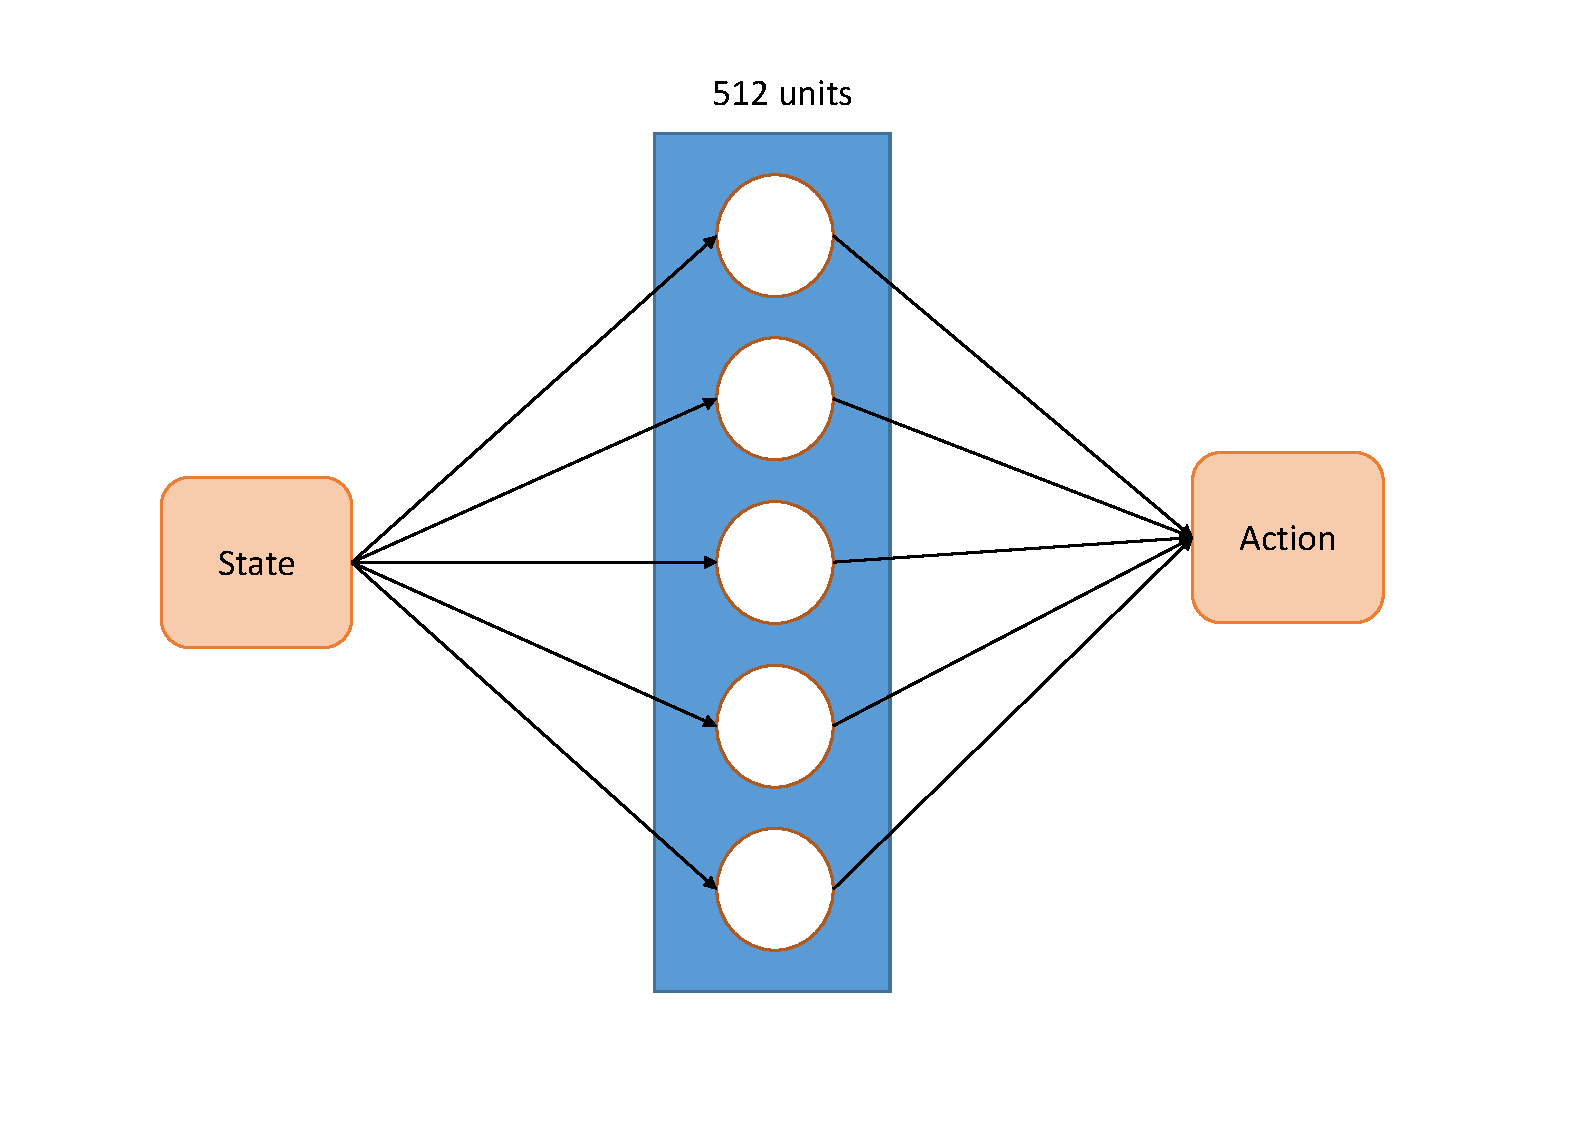
\includegraphics[height=80mm,width=140mm]{Pic/baseline/baseline_archetect.pdf}
    \caption[Cấu trúc mô hình cơ sở]{\textit{Cấu trúc mô hình cơ sở}, sử dụng một lớp ẩn để ước lượng hàm chất lượng sau khi lấy đặc trưng đã được phân tích trước đó.}
    \label{fig:baseline_archetect}
\end{figure}
Nhóm tác giả sử dụng cấu trúc như hình \ref{baseline_model} được lấy ý tưởng từ \cite{DBLP:journals/corr/MnihKSGAWR13} khi trực tiếp thực hiện \word{Phân tích đặc trưng}{Feature Extraction}thay vì sử dụng CNN.
\vspace{1cm}
\section{Một số thử nghiệm được thực hiện}
\noindentÝ tưởng đơn giản nhất cho việc tối ưu các bước thực hiện trong mỗi tập là thay đổi hàm phần thưởng thành một lượng âm. Khi đó, lượng phần thưởng âm này sẽ thúc đẩy robot mau chóng thắng nhưng nhóm tác giả có thể tiên lượng rằng robot sẽ không muốn tồn tại lâu trên bản đồ (thực hiện "kết liễu" càng nhanh càng tốt). Vì vậy giới hạn số bước có thể thực hiện trong một tập cũng là bước thử nghiệm trong phần này.\\
\\
Ngoài ra, khi hàm mất mát \ref{fig:baseline_loss} khá ổn định nhưng trung bình tích lũy \ref{fig:baseline_avg} không tăng tuyến tính như mong muốn. Chúng tôi giả thiết rằng bước khám phá chưa đủ đối với bài toán cụ thể này, do đó hai ý tưởng được đề xuất là tăng thêm số lượng bước thực hiện khám phá môi trường và tự tạo trạng thái tức ngẫu nhiên vị trí của robot và vị trí của vật cản.
\clearpage
\subsection{Mô hình đầu tiên}
\label{first_model}
Thực hiện các ý tưởng được nói ở trên, chúng tôi đề xuất các thay đổi cho mô hình mới như sau:
\begin{itemize}
    \item \textit{Thay đổi hàm phần thưởng:} Không chỉ sử dụng hai giá trị như mô hình cơ sở, chúng tôi xét môi trường robot hoạt động với mong muốn sẽ có một lượng phần thưởng âm khi robot đến càng gần điểm đích:
    \begin{subnumcases}{r(s_t,a_t,s_{t+1})=}
        +R_{0} & $s_{t+1}=\text{đích}$ \\
        -R_{1} & $s_{t+1}=\text{chết}$\\
        -d(s_{t+1}) & còn lại\label{first_subtract}
    \end{subnumcases}
    Với $R_0$ và $R_1$ là hằng số và hàm $d(s_{t+1})$ chỉ thị cho mối tương quan giữa trạng thái tiếp theo đến các vùng kết thúc, nhóm tác giả sử dụng ở đây là:
    \begin{equation}
        d(s_{t+1}) = \frac{\text{vị trí cột đích}-\text{vị trí cột trạng thái tiếp theo}}{\text{\text{vị trí cột đích} - \text{vị trí cột bắt đầu}}}
    \end{equation}
    Sở dĩ công thức \ref{first_subtract} phải trừ đi lượng\textit{ vị trí cột đích - vị trí cột bắt đầu} vì khi để giá trị cao quá sẽ khiến cho robot không còn muốn tồn tại trên bản đồ. Với cách định nghĩa như trên, nhóm tác giả mong muốn robot sẽ nhận biết được càng đến gần đích thì sẽ trừ càng ít và càng sử dụng nhiều số bước sẽ càng bị phạt.
    \item \textit{Thay đổi các khám phá môi trường:} Việc thử hiện hành động ngẫu nhiên theo chiến thuật \ref{e-greedy} dường như không đủ trường hợp thắng để robot có thể nhận biết được môi trường hiện tại có thể thắng hay không. Hình \ref{fig:agent_pos} đầu tiên cho thấy rằng rất khó để robot có thể vượt qua được các cột đầu tiên của môi trường và chiến thắng là điều trăn trở. Chứng tỏ đây là môi trường nhỏ rất dễ bước vào trạng thái kết liễu, do đó việc robot chỉ ngẫu nhiên thực hiện các bước có thể gói gọn trong vùng gần an toàn. Nhóm tác giả đề xuất thực hiện khởi tạo ngẫu nhiên vị trí của robot và vật cản để các trường hợp có thể gặp đa dạng hơn, từ đó có thể học được tốt hơn.
    \item \textit{Thay đổi cấu trúc của mô hình:} Thay vì sử dụng lớp ẩn 512 phần tử, mô hình mới chỉ sử dụng lớp ẩn 64 phần tử. Vì trạng thái hiện tại của môi trường rất nhỏ chỉ 14 giá trị do đó việc sử dụng lớp ẩn quá lớn là không cần thiết.
\end{itemize}
\begin{figure}[ht]
    \centering
    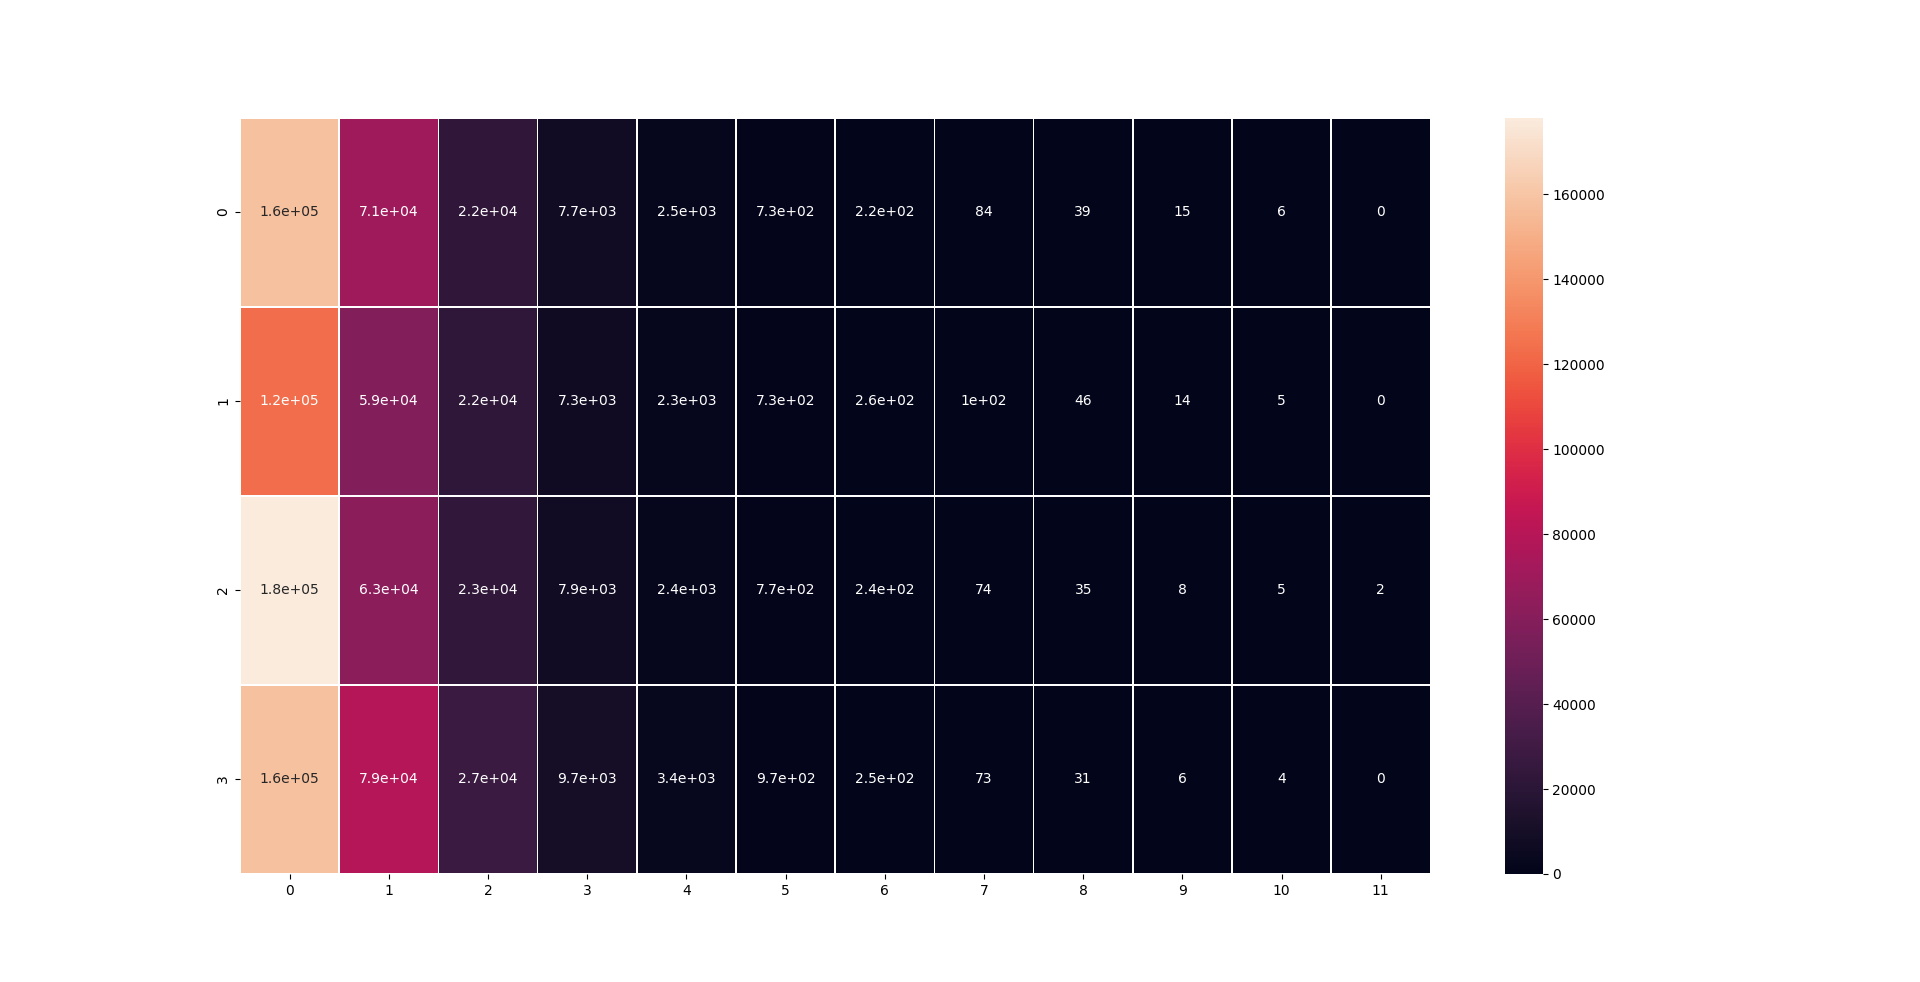
\includegraphics[width=1.2\linewidth]{Pic/First_model/agent_pos_before.png}
    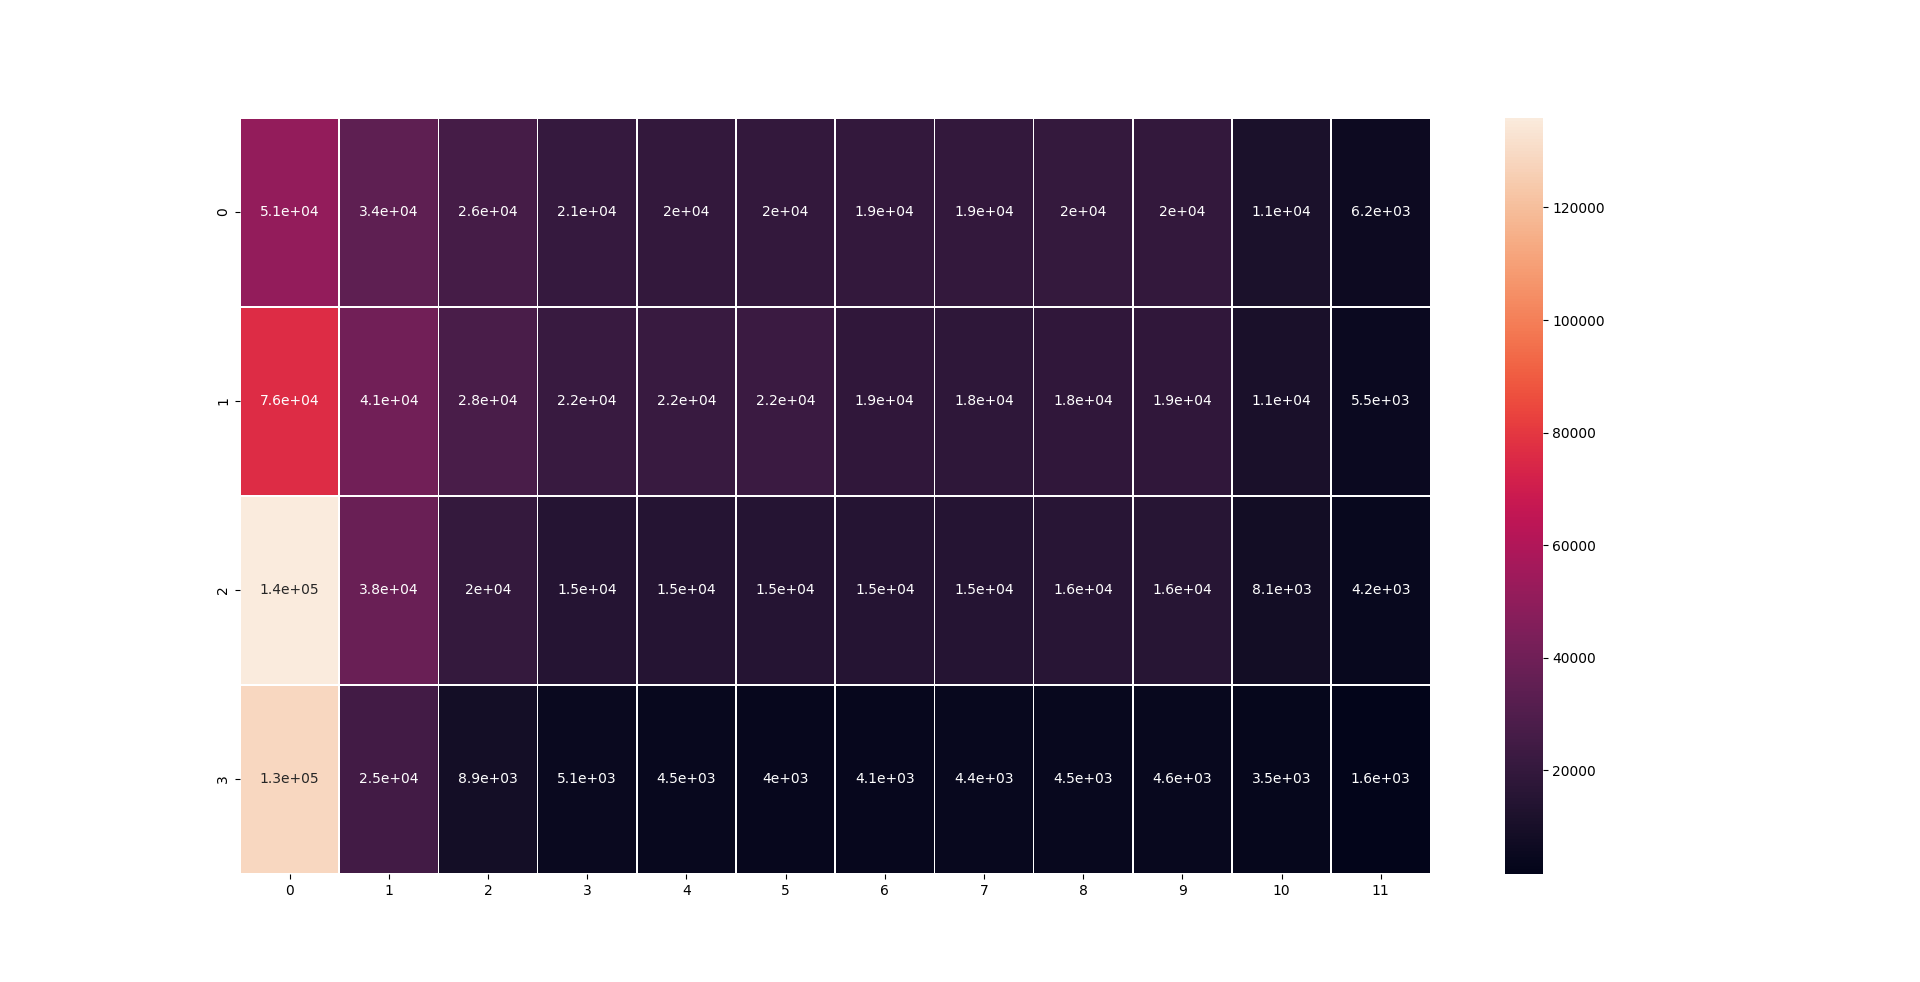
\includegraphics[width=1.2\linewidth]{Pic/First_model/agent_pos_after.png}
    \caption[Bản đồ nhiệt các vị trí robot thường xuất hiện]{Đây là kết quả của thử nghiệm chạy 1M bước ngẫu nhiên robot có thể đi được trong môi trường. Hình đầu tiên là kết quả không ngẫu nhiên vị trí robot, còn hình thứ hai là thực hiện khám phá môi trường khi ngẫu nhiên vị trí của các vật thể trong bản đồ. Có thể thấy được rằng các vị trí gần đích robot đã đi nhiều hơn từ đó tạo các dữ liệu thắng
    hơn cho mô hình.}
    \label{fig:agent_pos}
\end{figure}
\clearpage
\subsection{Mô hình thứ 2}\label{second_model}
Sau khi không có cải thiện trong mô hình \ref{first_model}, nhóm tác giả đưa ra giả thiết rằng các đặc trưng hiện tại khi đưa vào Q-learning chưa đủ liên quan với nhau để mô hình có thể nhận biết được tốt chúng. Ngoài ra các hàm mất mát của các kết quả \ref{first_model:first_try} và \ref{first_model:second_try} tuy có thể "hội tụ" nhưng đồ thị đồ thị phần thưởng tích lũy không tăng lên, có thể khẳng định rằng mô hình đã tìm đến điểm "cận cực đại" để khắc phục vấn đề này chúng tôi sử dụng \word{Công cụ tối ưu}{Optimizer}khác. 
\begin{itemize}
    \item \textit{Thay đổi cấu trúc của mô hình:} Từ 1 lớp ẩn 64 chúng tôi sử dụng 2 \word{Lớp ẩn}{Hidden layer} 64 nhằm giúp mô hình học được sự phức tạp của môi trường.
    \item \textit{Thay đổi công cụ tối ưu:} Nhóm tác giả thực hiện thay đổi từ RMSprop sang Adam.
    \item \textit{Thay đổi kích thước \word{cụm dữ liệu}{batch}:}  Theo  \cite{DBLP:journals/corr/abs-1803-02811}, sử dụng batch trong khoảng từ $32-2048$ là hợp lý đối với Q-learning. Do đó, chúng tôi lấy kết quả tốt nhất được thử nghiệm là 512 để thực hiện vào mô hình.
\end{itemize}
\begin{figure}[h]
    \centering
    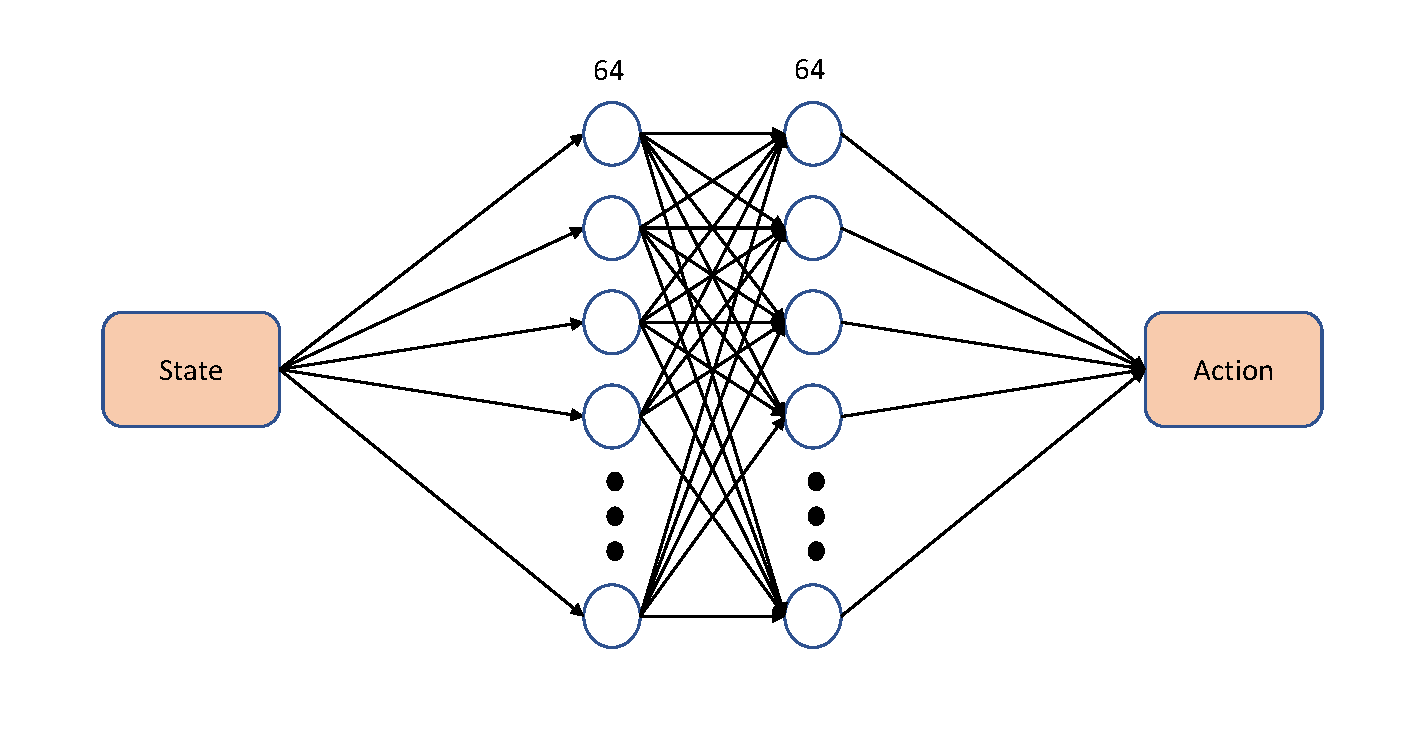
\includegraphics[width=\linewidth]{Pic/Second_model/second_arch.pdf}
    \caption[Cấu trúc của mô hình thứ hai]{\textit{Cấu trúc của mô hình thứ hai}, mô hình thêm một lớp ẩn nhằm thay đổi cách lớp ẩn thứ 2, tức Q-learning, nhìn vào trạng thái của môi trường.}
    \label{fig:second_arch}
\end{figure}
